\documentclass{bioinfo}

% For \addlinespace and \bottomrule
\usepackage{booktabs}

% Place the caption above the table
\usepackage{float}
\floatstyle{plaintop}
\restylefloat{table}

\copyrightyear{2014}
\pubyear{2014}
\application % applications note

\begin{document}
\firstpage{1}

\title[UniqTag]{
UniqTag: Content-derived unique and stable identifiers for gene annotation}
\author[Jackman \textit{et al.}]{
Shaun Jackman$^{1,2,*}$, Joerg Bohlmann$^{3,4}$ and \.{I}nan\c{c} Birol$^{1,5}$
\footnote{to whom correspondence should be addressed}
}

\address{
$^1$Genome Sciences Centre, British Columbia Cancer Agency, Vancouver, BC, Canada
\\$^2$Graduate Program in Bioinformatics, University of British Columbia, Vancouver, BC, Canada
\\$^3$Michael Smith Laboratories, University of British Columbia, Vancouver, BC, Canada
\\$^4$Department of Forest Sciences, University of British Columbia, Vancouver, BC, Canada
\\$^5$Department of Medical Genetics, University of British Columbia, Vancouver, BC, Canada
}

\history{Received on XXXXX; revised on XXXXX; accepted on XXXXX}

\editor{Associate Editor: XXXXXXX}

\maketitle

\begin{abstract}
\section{Summary}\label{summary}

When working on an ongoing genome sequencing and assembly project, it is
rather inconvenient when gene identifiers change from one build of the
assembly to the next. The gene labelling system described here, UniqTag,
addresses this common challenge. UniqTag assigns a unique identifier to
each gene that is a representative \emph{k}-mer, a string of length
\emph{k}, selected from the sequence of that gene. Unlike serial
numbers, these identifiers are stable between different assemblies and
annotations of the same data without requiring that previous annotations
be lifted over by sequence alignment. We assign UniqTag identifiers to
nine builds of the Ensembl human genome spanning seven years to
demonstrate this stability.

\section{Availability and
implementation}\label{availability-and-implementation}

The implementation of UniqTag is available at

\texttt{https://github.com/sjackman/uniqtag}

Supplementary data and code to reproduce it is available at

\texttt{https://github.com/sjackman/uniqtag-paper}

\section{Contact}\label{contact}

Shaun Jackman \textless{}sjackman@bcgsc.ca\textgreater{}

Inanc Birol \textless{}ibirol@bcgsc.ca\textgreater{}

\end{abstract}\section{Introduction}\label{introduction}

The task of annotating the genes of a genome sequence often follows
genome assembly. These annotated genes are assigned unique identifiers
by which they can be referenced. Assembly and annotation is often an
iterative process, by refining the method or by the addition of more
sequencing data. These gene identifiers would ideally be stable from one
assembly and annotation to the next. Serial numbers are used for
identifiers of genes annotated by software such as MAKER
(\href{http://dx.doi.org/10.1104/pp.113.230144}{Campbell, 2014}), which,
although certainly unique, are not stable between assemblies. A single
change in the assembly can result in a total renumbering of the
annotated genes.

One solution to stabilize identifiers is to assign them based on the
content of the gene sequence. A cryptographic hash function such as SHA
(Secure Hash Algorithm)
(\href{http://www.nist.gov/manuscript-publication-search.cfm?pub_id=910977}{Dang,
2012}) derives a message digest from the sequence, such that two
sequences with the same content will have the same message digest, and
two sequences that differ will have different message digests. If a
cryptographic hash were used to identify a gene, the same gene in two
assemblies with identical content would be assigned identical
identifiers. Yet, by design a slight change in the sequence, such as a
single-character substitution, would result in a completely different
digest.

Locality-sensitive hashing, in contrast to a cryptographic hash
function, aims to assign items that are similar to the same hash bucket.
A hash function that, after a small perturbation of the sequence,
assigns an identical identifier to the sequence is desirable for
labelling the genes of a genome annotation project. One such
locality-sensitive hash function, MinHash, was employed to identify web
pages with similar content
(\href{http://dx.doi.org/10.1109/SEQUEN.1997.666900}{Broder, 1997}) by
selecting a small representative set of words from the web page.
UniqTag, inspired by MinHash, selects a single representative
\emph{k}-mer from the sequence to assign a stable identifier to a gene.
These identifiers are intended for systematic labelling of genes rather
than assigning a biological name, which is typically based on biological
function or homology to orthologous genes.

\section{Description}\label{description}

A UniqTag can be generated from the nucleotide sequence of a gene or the
translated peptide sequence of a protein-coding gene. Using the peptide
sequence results in a UniqTag that is stable across synonymous changes
to the coding sequence as well as to changes in the untranslated regions
and introns of the gene. Since the amino acid alphabet is larger than
the nucleotide alphabet, fewer characters are required for a
\emph{k}-mer to be likely unique, resulting in an aesthetically pleasing
shorter identifier.

When two gene models have identical \emph{k}-mer compositions, they
would be assigned the same UniqTag. It is also possible that two genes
that have no unique \emph{k}-mer and similar \emph{k}-mer composition
are assigned the same UniqTag. In such cases, genes that have the same
UniqTag are distinguished by adding a numerical suffix to the UniqTag.

The UniqTag is designed to be stable but will change when the locus of
the UniqTag itself changes, or when a least-frequent \emph{k}-mer that
is lexicographically smaller than the previous UniqTag is created, or
when a duplicate \emph{k}-mer is created elsewhere that results in the
previous UniqTag no longer being a least-frequent \emph{k}-mer.

Concatenating two gene models results in a gene whose UniqTag is the
minimum of the two previous UniqTags, unless the new UniqTag spans the
junction of the two sequences. Similarly when a gene model is split in
two, one gene is assigned a new UniqTag and the other retains the
previous UniqTag, unless the previous UniqTag spanned the junction.
Importantly, unlike naming the genes after the genomic contigs or
scaffolds in which they are found, changing the order of the genes in a
genome assembly has no effect on the UniqTag.

\subsection*{Algorithm}\label{algorithm}
\addcontentsline{toc}{subsection}{Algorithm}

Here we define the UniqTag mathematically. Let $\Sigma$ be an alphabet,
such as the twenty standard amino acids or the four nucleotides. Let
$\Sigma^k$ be the set of all strings over $\Sigma$ of length \emph{k}.
Let \emph{s} be a string over $\Sigma$, such as the peptide or
nucleotide sequence of a gene. Let $C(s)$ be the set of all substrings
of \emph{s}, and $C_k(s)$ be the set of all \emph{k}-mers of \emph{s},
that is, all substrings of \emph{s} with length \emph{k}.

\[
C_k(s) = C(s) \cap \Sigma^k
\]

Let \emph{S} be a set of strings over $\Sigma$, such as the peptide or
nucleotide sequences of the annotated genes of a genome assembly. Let
$f(t, S)$ be the frequency in \emph{S} of a \emph{k}-mer \emph{t},
defined as the number of strings, or genes, in \emph{S} that contain the
\emph{k}-mer \emph{t}.

\[
f(t, S) = \left\vert \{ s \mid t \in C(s) \wedge s \in S \} \right\vert
\]

Let \emph{T} be the set of \emph{k}-mers of a string \emph{s}, and
$\min T$ be the lexicographically minimal \emph{k}-mer of \emph{T}. If
the \emph{k}-mers of \emph{T} were sorted alphabetically, it would be
the first \emph{k}-mer in the list.

Finally, $u_k(s, S)$ is the UniqTag, the lexicographically minimal
\emph{k}-mer of those \emph{k}-mers of \emph{s} that are least frequent
in \emph{S}. Typically, it is the first \emph{k}-mer in an
alphabetically sorted list of the \emph{k}-mers of a gene that are
unique to that gene.

\[
u_k(s, S) = \min \mathop{\arg\,\min}\limits_{t \in C_k(s)} f(t, S)
\]

\section{Results}\label{results}

To demonstrate the stability and utility of UniqTag, we assigned
identifiers to the genes of nine builds of the Ensembl human genome
(\href{http://dx.doi.org/10.1093/nar/gkt1196}{Flicek, 2014}) spanning
seven years and two major genome assemblies, NCBI36 up to build 54 and
GRCh37 afterward. An identifier of nine peptides ($k=9$) was assigned to
the first protein sequence, that with the smallest ENSP number, of each
gene. The number of common UniqTag identifers between older builds, from
build 40 to build 74, and the current build 75 is shown in Figure~1.
Also shown is the number of common gene and protein identifiers (ENSG
and ENSP accession numbers) between builds and the number of genes with
identical peptide sequences between builds. Although less stable than
the gene ID, the UniqTag is more stable than the protein ID and the
peptide sequence.

Whereas the gene and protein identifiers can, with effort, be lifted
over from older builds to the newest build, the UniqTag identifier can
be generated without any knowledge of previous assemblies, making it a
much simpler operation. The number of identical peptide sequences
between builds shows the stability that would be expected of using a
message digest, such as SHA, of the peptide sequence as the identifier.
Supplementary figure~S1 shows that the UniqTag stability is insensitive
to the size of the UniqTag identifier for values of \emph{k} between 8
and 50 peptides. The data for these figures are shown in supplementary
table~S1.

\begin{figure}[htbp]
\centering
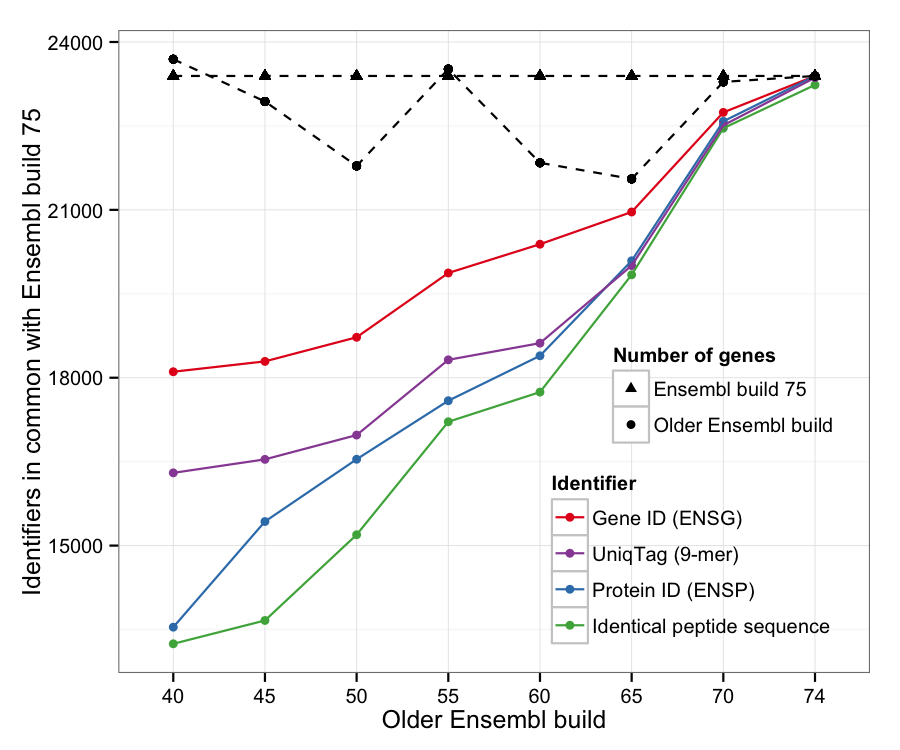
\includegraphics{ensembl.png}
\caption{The number of common UniqTag identifers between older builds of
the Ensembl human genome and the current build 75, the number of common
gene and protein identifiers between builds, and the number of genes
with identical peptide sequences between builds.}
\end{figure}

\section*{Acknowledgements}\label{acknowledgements}
\addcontentsline{toc}{section}{Acknowledgements}

The author thanks Nathaniel Street for his enthusiastic feedback, the
SMarTForests project and the organizers of the 2014 Conifer Genome
Summit that made our conversation possible.

\emph{Funding}: This work was supported by the Natural Sciences and
Engineering Research Council of Canada, Genome British Columbia, Genome
Alberta, Genome Quebec and Genome Canada.

\section*{References}\label{references}
\addcontentsline{toc}{section}{References}

\href{http://dx.doi.org/10.1109/SEQUEN.1997.666900}{Broder, A. Z.
(1997)} On the resemblance and containment of documents.
\emph{Compression and Complexity of Sequences}, 1997 Proceedings,
21-29.\\\href{http://dx.doi.org/10.1104/pp.113.230144}{Campbell, M. S.
\emph{et al.} (2014)} MAKER-P: a tool-kit for the rapid creation,
management, and quality control of plant genome annotations. \emph{Plant
Physiology}, 164(2),
513-524.\\\href{http://www.nist.gov/manuscript-publication-search.cfm?pub_id=910977}{Dang,
Q. H. (2012)} Secure Hash Standard (SHS). \emph{NIST FIPS}, 180(4),
1-35.\\\href{http://dx.doi.org/10.1093/nar/gkt1196}{Flicek, P. \emph{et
al.} (2014)} Ensembl 2014. \emph{Nucleic Acids Research}, 42(D1),
D749-D755.
\end{document}
